\section{Basin-aware gain scheduling}\label{sec:basin-aware}

This section turns the tolerated disturbance into a design requirement (details: Supplementary Material, Section~\ref{S-supp:ba}).

\subsection{Formulation}\label{sec:ba-form}

At a spindle speed $n$, a gain $g$ and a depth $a$ are admissible if
\begin{equation}\label{eq:admissible}
  a<\alim(n,g),\quad \bar b(n,a,g)\le(1-\rho)\Vmax,\quad \beta(n,a,g)\ge\beta_{\mathrm{req}},\quad a\le a_{\mathrm{cap}},
\end{equation}
that is, if the cut is linearly stable, keeps a voltage margin $\rho$ in its forced command, has a certified kick $\beta$ (C2, averaged collocation model, Section~\ref{sec:cert-c2}) of at least the required disturbance tolerance $\beta_{\mathrm{req}}$, an instantaneous velocity perturbation at any phase of the tooth period, and does not exceed an assumed depth cap $a_{\mathrm{cap}}$. The certificate is computed for the nominal forced command with the full clip. The basin-aware depth is
\begin{equation}\label{eq:arob}
  a_{\mathrm{rob}}(n;\beta_{\mathrm{req}})=\max_{g\in\mathcal G}\max\bigl\{a\in\mathcal A:\text{ all }a'\in\mathcal A\text{ with }a'\le a\text{ admissible with }g\bigr\},
\end{equation}
with $\mathcal A$ a grid of depths and $\mathcal G$ the gains evaluated by the search; $a_{\mathrm{rob}}$ and its gain, the basin-aware gain $g_{\mathrm{rob}}$, are a grid optimum. Here $\rho=0.1$ and $a_{\mathrm{cap}}=2D=\SI{32}{\milli\metre}$, an assumption: the case study gives neither the cutting length of the tool nor the mode shape over such depths, and tested up to \SI{10}{\milli\metre}.
% src: verification/paper/basin_aware.py/.json (protocol: rho 0.1, a_phys 32 mm); results/cuts_main.json (deepest published cut 10 mm)

\subsection{The basin-aware stability chart}\label{sec:ba-res}

Figure~\ref{fig:ba} shows the chart at 21 speeds from 500 to \SI{3000}{\rpm}, for gains of 0--\SI{3000}{\volt\second\per\metre} on a refined grid and depths on a \SI{2}{\milli\metre} grid. Certificates scanned with a reduced collocation order were certified again with the default order at every design point and every lower depth with a kick below $1.15\,\beta_{\mathrm{req}}$.
% src: verification/paper/basin_aware.py/.json (protocol: GRID_RPM 500:125:3000, G_COARSE 0:250:3000 with refinement +-125, +-62.5, DEPTHS 2:2:32 mm, rho 0.1, a_phys 32 mm, BETA_REQ 1, 2, 5 mm/s; nred_vs_default: reduced/default 0.994-1.044)

First, the linear limit at the chosen gain, not the voltage, binds at most speeds (15, 17 and 15 of the 21 speeds for $\beta_{\mathrm{req}}=1$, 2 and \SI{5}{\milli\metre\per\second}), the certificate at six speeds for \SI{5}{\milli\metre\per\second}. Second, the basin-aware gain is never above the gain of the authority rule with the same range and voltage margin (median ratio 0.94, 0.85 and 0.72; Fig.~\ref{fig:ba}c). Third, the chart keeps no explicit margin below the linear limit (median ratio of $a_{\mathrm{rob}}$ to $\alim(g_{\mathrm{rob}})$ 0.97, 0.97 and 0.91).
% src: verification/paper/basin_aware.json (summary.1/2/5: primary_binding_counts_grid21 {linear 15, a_phys 6}, {linear 17, a_phys 3, certificate 1}, {linear 15, certificate 6}; fair_designs.json speeds.*.auth10.g against g_star_by_rpm: never below it, median ratio g_rob/g_auth10 0.941/0.846/0.716 (recomputed); per_speed.*.designs.*.a_rob_over_a_lim_at_g median 0.973/0.970/0.909 over the 21 speeds, recomputed)

\begin{table}[!tbp]
  \centering
  \caption{The basin-aware chart and the reference schedules at the 21 speeds of the chart, all with $g\le\SI{3000}{\volt\second\per\metre}$ except the former reference. Depth: operating depth, $\achk=\min\{0.9\,\alim,a_{\mathrm{TD}}\}$ for the references, $a_{\mathrm{rob}}$ for the chart; step: the largest depth up to which the step entry from rest also settles; certifiable: the depth up to which the design's own gain meets the chart's conditions for $\beta_{\mathrm{req}}=1$, 2 and \SI{5}{\milli\metre\per\second}; $\bar b$: rigorous bound on the forced command; $\beta$ and $\Delta v^*$: certified kick (C2, default collocation order) and simulated critical kick (smallest of four phases, infinite where no kick up to \SI{3}{\metre\per\second} causes chatter) at the operating depth. Depths are means over the speeds, $\bar b$ medians (largest) and kicks medians (smallest).}
  \label{tab:ba}
  \footnotesize
  \setlength{\tabcolsep}{3pt}
  \begin{tabular}{@{}lcccccc@{}}
    \toprule
    Design & Depth & Step & Certifiable (\si{\milli\metre}) & $\bar b$ & $\beta$ & $\Delta v^*$\\
     & (\si{\milli\metre}) & (\si{\milli\metre}) & 1 / 2 / \SI{5}{\milli\metre\per\second} & (\si{\volt}) & (\si{\milli\metre\per\second}) & (\si{\milli\metre\per\second})\\
    \midrule
    Published, Eq.~\eqref{eq:pub} & 11.3 & 11.3 & 9.3 / 9.3 / 9.0 & 3.1 (9.9) & 11.0 (0.0) & 57.1 (20.0)\\
    Authority, no margin & 17.1 & 17.1 & 9.0 / 8.1 / 5.2 & 4.6 (9.0) & 6.3 (0.0) & 15.4 (10.5)\\
    Authority, \SI{10}{\percent} margin & 16.8 & 16.8 & 21.2 / 18.2 / 9.8$^{a}$ & 4.6 (8.1) & 7.9 (0.8) & 15.1 (10.5)\\
    Former ref., $g\le1500$ & 15.5 & 15.5 & 10.9 / 10.9 / 9.5 & 2.5 (9.0) & 8.5 (0.0) & 17.5 (10.8)\\
    \addlinespace
    Chart, \SI{1}{\milli\metre\per\second} & 21.7 & 16.1 & 21.7 / -- / -- & 4.8 (7.7) & 4.3 (1.2) & 8.1 (2.5)\\
    Chart, \SI{2}{\milli\metre\per\second} & 19.9 & 15.8 & -- / 19.9 / -- & 4.8 (6.7) & 5.0 (2.0) & 10.1 (3.9)\\
    Chart, \SI{5}{\milli\metre\per\second} & 16.0 & 15.1 & -- / -- / 16.0 & 4.0 (6.6) & 7.2 (5.2) & 15.4 (10.4)\\
    \addlinespace
    \multicolumn{7}{@{}l}{\emph{With the depth margin $a\le0.9\,\alim$ also in the chart}}\\
    Chart, \SI{1}{\milli\metre\per\second} & 19.7 & 15.7 & 19.7 / -- / -- & 5.3 (7.8) & 4.3 (1.0) & 16.4 (4.2)\\
    Chart, \SI{2}{\milli\metre\per\second} & 18.8 & 15.4 & -- / 18.8 / -- & 4.8 (7.1) & 6.0 (2.1) & 12.7 (7.0)\\
    Chart, \SI{5}{\milli\metre\per\second} & 15.1 & 14.4 & -- / -- / 15.1 & 4.0 (7.0) & 7.0 (5.0) & 17.1 (11.5)\\
    Authority, \SI{10}{\percent} margin & 16.8 & 16.8 & 19.6 / 17.1 / 9.4$^{a}$ & \multicolumn{3}{c}{as above}\\
    \bottomrule
  \end{tabular}

  \smallskip
  \parbox{0.95\textwidth}{\footnotesize $^{a}$\,With a tolerance of \SI{10}{\milli\volt} on the \SI{8.1}{\volt} test, which the rigorous bound of this gain exceeds by at most \SI{2.3}{\milli\volt} at one grid depth at five speeds (Supplementary Material, Section~\ref{S-supp:std-ba-compare}); counted strictly, 17.9 / 15.5 / \SI{9.2}{\milli\metre} and 16.6 / 14.6 / \SI{8.9}{\milli\metre}.}
\end{table}
% src: verification/paper/ref_under_ba_tol.py/.json (summary.auth10: tol_k1 21.24/18.19/9.81, tol_k0.9 19.62/17.14/9.43, strict_k1 17.90/15.52/9.24, strict_k0.9 16.57/14.57/8.86; speeds_changed 1250, 1375, 1500, 2375, 2500; ref_under_ba_cache.jsonl bbar 8.1005-8.1023 V at 4 or 6 mm there; chart_rows_with_8p1_lt_bbar_le_8p11: none; other references unchanged)
% src: verification/paper/fair_designs.py/.json (summary.mean_a_chk_mm pub 11.34, auth0 17.13, auth10 16.77, auth1500 15.50); verification/paper/ref_under_ba.py/.json (summary: pub 9.33/9.33/8.95, auth0 8.95/8.10/5.24, auth10 17.90/15.52/9.24, auth1500 10.86/10.86/9.52, ba 21.71/19.90/16.00) and ref_under_ba_kappa0.9.json (auth10 16.57/14.57/8.86, ba 19.71/18.76/15.14); verification/paper/ba_kappa.py/.json (summary mean_a_rob_mm 19.71/18.76/15.14); verification/paper/ba_entry.json and ba_entry_kappa.json (summary mean_a_step_mm 16.10/15.81/15.14 and 15.71/15.43/14.38); verification/paper/table6.py/.json (bbar, beta, crit from fair_compare.json summary: pub 3.06 (9.90), 11.02 (0.00), 57.06 (19.96); auth0 4.63 (9.00), 6.26 (0.00), 15.39 (10.53); auth10 4.63 (8.08), 7.92 (0.84), 15.06 (10.53); auth1500 2.53 (9.00), 8.546 (0.00), 17.52 (10.76); ba1 4.84 (7.71), 4.27 (1.23), 8.12 (2.55); ba2 4.84 (6.68), 4.97 (2.02), 10.09 (3.93); ba5 4.03 (6.55), 7.20 (5.23), 15.39 (10.42); depth margin from ba_kappa.json beta_ref_at_a_rob and bak_crit.json: 5.33 (7.77), 4.27 (1.04), 16.42 (4.20); 4.84 (7.08), 5.96 (2.09), 12.66 (6.98); 4.03 (7.01), 6.98 (5.05), 17.15 (11.49))

\begin{figure}[!tbp]
  \centering
  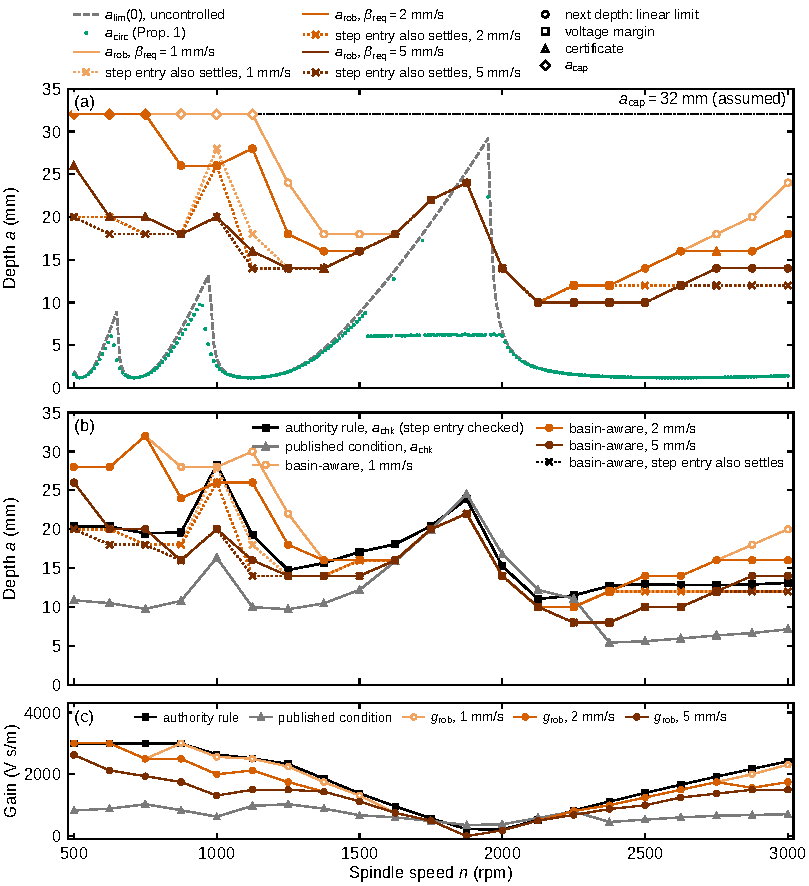
\includegraphics[width=0.86\textwidth]{figures/fig_basin_aware.pdf}
  \caption{Basin-aware stability chart at the 21 speeds (only the depths of the \SI{2}{\milli\metre} grid are certified). (a)~$a_{\mathrm{rob}}$ for $\beta_{\mathrm{req}}=1$, 2 and \SI{5}{\milli\metre\per\second} (certified kick of C2, averaged collocation model; \SI{10}{\percent} voltage margin), with the condition that fails at the next grid depth (markers); crosses: largest grid depth up to which the step entry from rest also settles in the simulator with the same gain (verified numerically, not certified); $\alim(0)$: uncontrolled limit; $a_{\mathrm{circ}}$: depth below which the averaged delay model attracts every solution at the gains of Section~\ref{sec:feasibility} (Proposition~\ref{prop:circle}; not computed at the chart's gains); $a_{\mathrm{cap}}$: assumed depth cap. (b)~Same gain range ($g\le\SI{3000}{\volt\second\per\metre}$) and depth margin ($a\le0.9\,\alim$): basin-aware depth (circles), its step-entry depth (crosses) and step-entry-checked depths $\achk$ of the authority rule with the same \SI{10}{\percent} voltage margin, Eq.~\eqref{eq:feas}, and of the published condition, Eq.~\eqref{eq:pub}, which has none. (c)~Gains of the chart of (a), of the authority rule with the \SI{10}{\percent} margin and of the published condition.}
  \label{fig:ba}
\end{figure}

\subsection{Comparison with the reference schedules}\label{sec:ba-compare}

Table~\ref{tab:ba} compares the chart with reference schedules computed with the same gain range, except the former schedule of Section~\ref{sec:feasibility} ($g\le\SI{1500}{\volt\second\per\metre}$), and operating at the checked depth $\achk$ of Eq.~\eqref{eq:achk}. Judged by the chart's own conditions, the authority gain with the same voltage margin keeps every grid depth admissible up to 21.2, 18.2 and \SI{9.8}{\milli\metre} on average for 1, 2 and \SI{5}{\milli\metre\per\second} (note $a$ of Table~\ref{tab:ba}: a numerical tie), against 21.7, 19.9 and \SI{16.0}{\milli\metre} for the basin-aware gain. With the depth margin $a\le0.9\,\alim$ imposed on the chart as well, the choice of the gain matters little for \SI{1}{\milli\metre\per\second}, where the authority gain certifies as deep, and much for \SI{5}{\milli\metre\per\second}, where it certifies \SI{5.7}{\milli\metre} less: the authority rule spends the voltage on raising the linear limit, the chart keeps the residual authority that a larger disturbance needs. Against the authority rule's own operating depth (\SI{16.8}{\milli\metre}), the chart with the depth margin is 2.9 and \SI{2.0}{\milli\metre} deeper for 1 and \SI{2}{\milli\metre\per\second} and \SI{1.6}{\milli\metre} shallower for \SI{5}{\milli\metre\per\second}.
% src: verification/paper/fair_designs.json (summary); verification/paper/ref_under_ba.json, ref_under_ba_kappa0.9.json (summary); verification/paper/ba_kappa.json (summary); ba_kappa.json summary.mean_a_rob_mm 19.71/18.76/15.14 against fair_designs.json mean_a_chk_mm.auth10 16.77: +2.94/+1.99/-1.63 mm

At their own operating depths the references keep larger certified kicks than the chart for 1 and \SI{2}{\milli\metre\per\second}, because they cut less deep; but the smallest certified kick of the authority gain over the grid depths below its operating depth and at it is \SI{2.3}{\milli\metre\per\second} (median) and reaches 1, 2 and \SI{5}{\milli\metre\per\second} at 20, 18 and 5 of the 21 speeds, whereas the chart certifies $\beta_{\mathrm{req}}$, on the averaged collocation model, at every grid depth up to $a_{\mathrm{rob}}$.
% src (kicks at the operating depth): verification/paper/fair_compare.py/.json (summary.auth10: beta_range median 2.29 (minimum over the grid depths below a_op and a_op itself), beta_range_at_least 1/2/5: 20/18/5 of 21; checks.recheck: stored kick and certificate recomputed bit for bit)

The assumed cap binds at 6, 3 and 0 of the 21 speeds, but the deep cuts it admits carry much of the depth advantage: with caps of 16 and \SI{10}{\milli\metre} the chart gains at most \SI{0.6}{\milli\metre} mean depth over the authority rule capped the same way (\SI{0.5}{\milli\metre} less for \SI{5}{\milli\metre\per\second} with \SI{16}{\milli\metre}); it still gains certified disturbance: where both gains meet the chart's conditions up to the cap, the smallest certified kick over the grid depths is larger with the chart's gain by a median factor of 2.3 for \SI{10}{\milli\metre} (21 speeds) and 1.5 for \SI{16}{\milli\metre} (16 speeds), with the same voltage tolerance; the reference gains are judged with the reduced collocation order, which overstates the default-order kick by up to \SI{12}{\percent}.
% src: verification/paper/ba_cap.py/.json (summary.per_cap.32.*.n_at_cap 6/3/0; per_cap.16.<b>.a_rob_minus_ref_capped_mean_mm.auth10 +0.60/+0.60/-0.55, per_cap.10 0.0); verification/paper/cap_kicks.py/.json and cap_kicks_tol.json (--tol: reference scans of ref_under_ba_tol.py; caps.<cap>.paired_both_at_cap: 10 auth10_vs_ba_1 n 21 median 2.30 (strict n 16, 2.09); 16 auth10_vs_ba_1 n 16 median 1.52 (strict n 13, 1.38); reduced over default order at the reference operating depths 0.975-1.122, median 1.008 (fair_compare.json per_speed beta_range at a_op against beta_op.fast_mmps, recomputed))

\subsection{Validation, entry and robustness}\label{sec:ba-valid}

At all 21 speeds the simulated critical kick of the design points, smallest over four phases, is at least 2.55, 1.97 and 2.08 times $\beta_{\mathrm{req}}$, and at six speeds kicks of exactly $\beta_{\mathrm{req}}$ at all 16 phases never caused chatter: in the simulator no design point has a smaller basin than required, along the kick direction.
% src: verification/paper/basin_aware.json (validation_summary.1/2/5: points 6, all_above_beta_req true, worst_crit_kick_over_beta_req_min 2.750/2.780/2.272, kicks_of_beta_req_chattering 0 of 96); verification/paper/fair_compare.json (summary.ba1/ba2/ba5.crit_kick_mmps.min 2.549/3.931/10.419, i.e. 2.55/1.97/2.08 times beta_req; crit_kick_unsettled 0)

The chart certifies the settled cut, not the entry: with its gains the face entry settles at every grid depth up to $a_{\mathrm{rob}}$, but the step entry only up to 16.1, 15.8 and \SI{15.1}{\milli\metre} on average (crosses in Fig.~\ref{fig:ba}a; simulated, not certified), so that with an abrupt entry saturation during the entry sets the usable depth, for the chart as for the authority rule, whose checked depth includes this check.
% src: verification/paper/ba_entry.py/.json (summary.*: n_a_face_below_a_rob 0; mean_a_step_mm 16.10/15.81/15.14)

Under the first 30 samples of the $\pm\SI{10}{\percent}$ error draw of Section~\ref{sec:delayed-robust} at the same six speeds, the failure probability at the designs' own depths (no settling, or chatter after a kick of $\beta_{\mathrm{req}}$ at one of four phases) is 16.7, 11.7 and \SI{10.0}{\percent} for the chart with the depth margin and 39, 39 and \SI{11}{\percent} without it, against \SI{6.7}{\percent} for the authority rule with the \SI{10}{\percent} margin; what matters is the ratio to the linear limit, 0.81--0.90 for the chart with the depth margin against 0.51--0.81 for the reference where its step-entry check binds and 0.90 at \SI{2000}{\rpm}. Of the chart's 69 failures with the depth margin, 55 are cuts whose sampled averaged model is linearly unstable: the errors consume mainly the margin to the linear limit, at \SI{2875}{\rpm} also the voltage margin, and only rarely the certified basin. These probabilities guarantee nothing; the chart needs margins that cover the errors of the model.
% src: verification/paper/mc_designs.py (protocol), mc_designs_kappa.json and mc_designs_chart.json (complete; summary.<b>.own: ref 12/180 (own); chart with margin own 30/21/18 of 180 (0.167/0.117/0.100); chart without margin own 71/71/19 (0.394/0.394/0.106)); mc_designs_kappa.json per_speed.<rpm>.b.<b>.own.BA: sums of unsettled_and_cf_unstable 21/20/14 (55)
